\documentclass[a4paper,12pt,titlepage]{report}
\usepackage[utf8]{inputenc}
\usepackage{graphicx}

\usepackage[footnotesize]{caption}

\makeatletter
\renewcommand{\fnum@figure}{\small\textbf{\figurename~\thefigure}}
\makeatother

\setcounter{secnumdepth}{-1} 

% Title Page
\title{Assignment Network Simulation}
\author{Peter De Wolf \& Wout Vekemans}
\begin{document}
\begin{titlepage}
	\maketitle
	\thispagestyle{empty}
\end{titlepage}

\section{Exercise 1: Bandwidth restrictions on Kotnet}
\begin{enumerate}
 \item When we leave out the uploading connection, the throughput of the download connection is relatively constant. See figure \ref{noUpload}. Sometimes a packet gets lost, decreasing the throughput.\\
  \begin{figure}[htb]
\centering
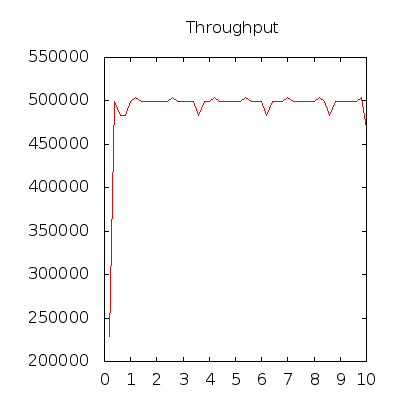
\includegraphics[width=0.5\textwidth]{noUpload.png}
\caption{Throughput of the main FTP connection}
\label{noUpload}
\end{figure}
\item When re-enabling the uploading connection, we see that the download rate drops when the upload starts. This is caused by the fact that the ACKs of the download need to travel through the same connection as the packets uploaded by the user. This results in a lot of dropped ACKs, which causes the server to restart sending, and therefore decreasing the throughput of the download link. See figure \ref{upAndDown}.\\
  \begin{figure}[htb]
\centering
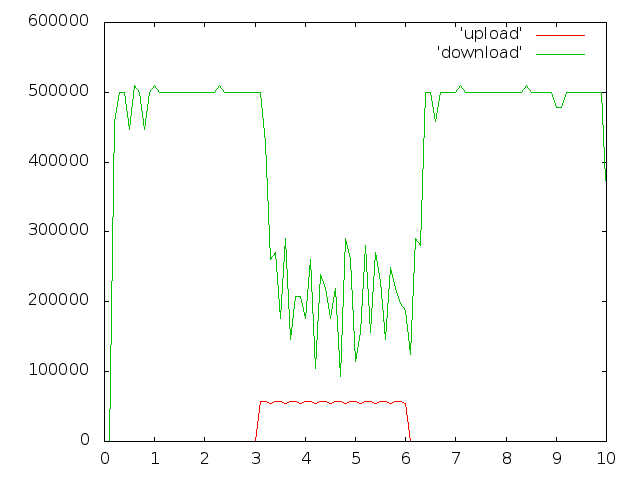
\includegraphics[width=0.5\textwidth]{withUpload.png}
\caption{Throughput of the FTP and UDP connection}
\label{upAndDown}
\end{figure}
\item When a fixed amount of upload bandwidth is allocated to both applications, there wont be a drop in the download throughput. It would be like there were to separate upload connections: one for the ACKs of the FTP connection, and one for the data packets of the CBR connection, so they would both have more or less constant throughput.\\
\end{enumerate}


\end{document}          
